\experiment{5}{%
    Compute the mean, median, and mode for a given dataset. Compare these measures and analyze which one best represents the data.
}

\subsection{Computing mean, median and mode}

\begin{lstlisting}[style=python]
import pandas as pd 
import matplotlib.pyplot as plt 
import numpy as np

df_student = pd.read_csv("dataset.csv", delimiter=',', header='infer')

sel = df_student[['Marks', 'StudyHours', 'Attendance']]

cal = pd.DataFrame({
    'Attribute': sel.mean().index,
    'Mean': sel.mean().values.round(2),
    'Median': sel.median().values.round(2),
    'Mode': sel.mode().iloc[0].values.round(2)
})

print(cal)
\end{lstlisting}

\textbf{Output:}

\begin{tabular}{ccccc}
    \toprule
    & \textbf{Attribute} & \textbf{Mean} & \textbf{Median} & \textbf{Mode} \\
    \midrule
    0 & Marks  & 70.20 & 74.5 & 35.0 \\
    1 & StudyHours  & 4.07 & 4.0 & 4.0 \\
    2 & Attendance  & 75.57 & 80.0 & 80.0 \\
    \bottomrule
\end{tabular}


\subsection{Representation}

\subsubsection*{i) Marks}

\begin{lstlisting}[style=python]
sturges = round(1+np.log2(df_student.Marks.count()))

plt.hist(df_student.Marks, bins=sturges, ec="white", zorder = 2)

plt.xlabel("marks")
plt.ylabel("no. of students")
plt.grid(zorder=0, linestyle=":", alpha=0.6)

plt.axvline(cal.Mean.iloc[0], color='#8EBA42', linestyle='--', label="mean")
plt.axvline(cal.Median.iloc[0], color='#D9534F', linestyle='-.', label="median")
plt.axvline(cal.Mode.iloc[0], color='#F59E0B', linestyle='-', label="mode")

plt.legend()
plt.show()

\end{lstlisting}

\textbf{Output:}

\begin{figure}[H]
    % \centering
    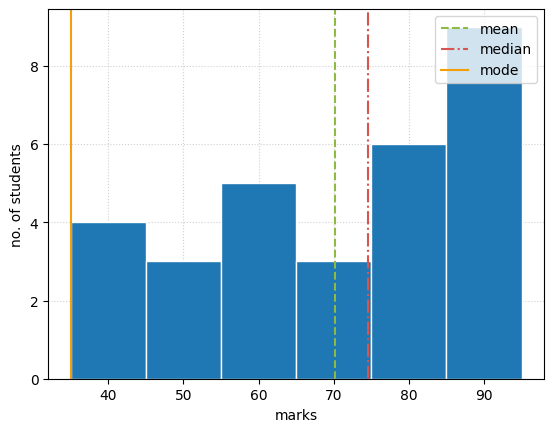
\includegraphics[width=0.75\textwidth]{img/exp5_markHist.png}
    % \caption{Marks of Each Student — Bar Chart}
    % \label{fig:marks_bar}
\end{figure}

\subsubsection*{ii) Study Hours}

\begin{lstlisting}[style=python]
plt.hist(df_student.StudyHours, bins=sturges, ec="white", zorder = 2)

plt.xlabel("study hours")
plt.ylabel("no. of students")
plt.grid(zorder=0, linestyle=":", alpha=0.6)

plt.axvline(cal.Mean.iloc[1], color='#8EBA42', linestyle='--', label="mean")
plt.axvline(cal.Median.iloc[1], color='#D9534F', linestyle='-.', label="median")
plt.axvline(cal.Mode.iloc[1], color='#F59E0B', linestyle='-', label="mode")

plt.legend()
plt.show()

\end{lstlisting}

\textbf{Output:}

\begin{figure}[H]
    % \centering
    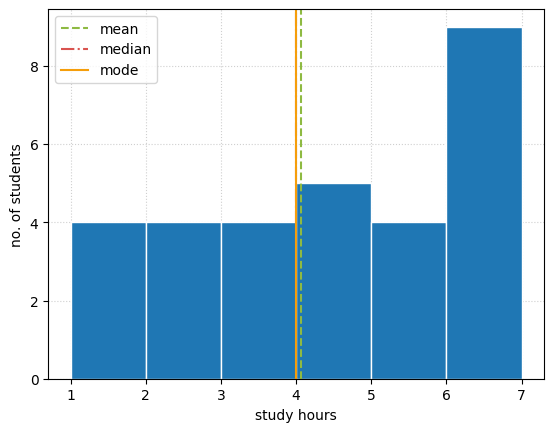
\includegraphics[width=0.75\textwidth]{img/exp5_studyhHist.png}
    % \caption{Marks of Each Student — Bar Chart}
    % \label{fig:marks_bar}
\end{figure}

\subsubsection*{iii) Attendance}

\begin{lstlisting}[style=python]
plt.hist(df_student.Attendance, bins=sturges, ec="white", zorder = 2)

plt.xlabel("attendance")
plt.ylabel("no. of students")
plt.grid(zorder=0, linestyle=":", alpha=0.6)

plt.axvline(cal.Mean.iloc[2], color='#8EBA42', linestyle='--', label="mean")
plt.axvline(cal.Median.iloc[2], color='#D9534F', linestyle='-.', label="median")
plt.axvline(cal.Mode.iloc[2], color='#F59E0B', linestyle='-', label="mode")

plt.legend()
plt.show()

\end{lstlisting}

\textbf{Output:}

\begin{figure}[H]
    % \centering
    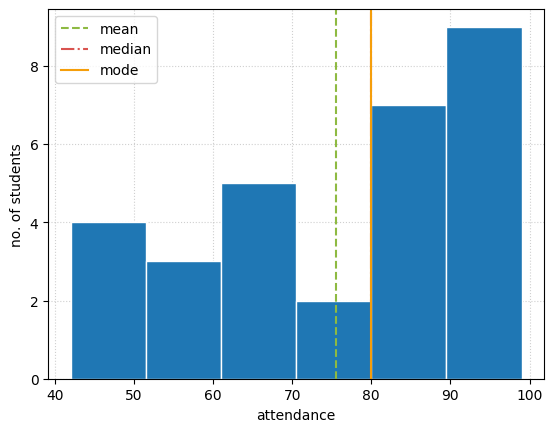
\includegraphics[width=0.75\textwidth]{img/exp5_attendanceHist.png}
    % \caption{Marks of Each Student — Bar Chart}
    % \label{fig:marks_bar}
\end{figure}

% 

% add one more graph of 3 bars beside one another for comapring mean median and mode at same time.

% 

\subsection{Observation}

i. For marks, the mean is lower than median, which confirms the left skewned distribution seen in above histogram. A few students with low marks are pulling the mean down.

ii. The mode of Marks is 35.0, which is nowhere close to mean or median of Marks, indicating it is not a true measure of central tendency for this column.

iii. For StudyHours, the mean, median and mode are nearly identical, suggesting a symmetrical distribution, which can be seen in the graphs above. Mean is a good representation here.

iv. For Attendance, mean is slighly lower than median and mode, indicating a very slight left skewness. 

v. Across all thress attributes, median the most reliable measure of central tendency.